\subsection{Checkpoint rounds}
In this section the steps involved in creating a checkpoint is discussed. The checkpoint creation is triggered at regular intervals. Since we are depending on the adapted Stabilizing ABC protocol, the checkpoint creation is proceeded to second step only if a majority of validators in the system are in agreement for creation. Checkpoint creation is completed in mainly three rounds and which are the following here:

\begin{itemize}
\item Choosing a validator
\item Agree on hash of checkpoint proposal
\item Agree on checkpoint proposal contents
\end{itemize}

\paragraph{}In an open system, we need to ensure that one participant is elected to propose a checkpoint and this can be verified by every other participant in the system. In the first step, one of the validators is chosen based on a priority value calculated individually by each validator. The priority values are calculated based on output of a VRF function. So every other validator in the system which can keeps track of the stake values in the system, can verify the calculated value and determine if a validator has send an honest value or not. The vote based on the VRF output is used to compare and determine the chosen validator. Tie in vote value is broken using the priority value, which is unique for each validator public key. So with the completion of the first round, the system finds a public key from which a checkpoint is expected to be proposed.\\
Further, in the second round, the chosen validator calculates a checkpoint data based on its local DAG and broadcasts the hash of this checkpoint. This is done so that every honest validator in the system can agree on a single checkpoint message contents and can discard the invalid messages right away. In the final step, the chosen validator broadcasts the actual contents of the checkpoint, and is checked and agreed by the validators. The finalised contents are then injected into the local DAG. 

\begin{figure}
    \centering
    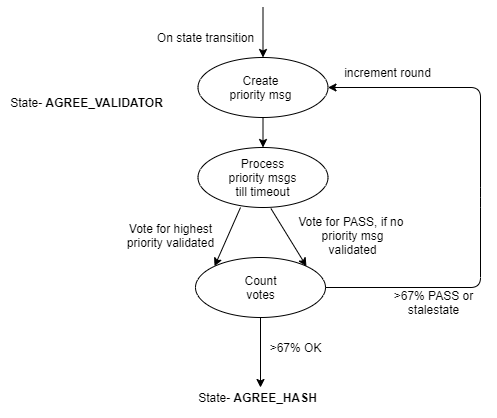
\includegraphics[width=100mm,scale=0.25]{figures/drawio/priority.png}
    \caption{AGREE VALIDATOR transition.}
    \label{fig:VALIDATOR}
\end{figure}


\begin{figure}
    \centering
    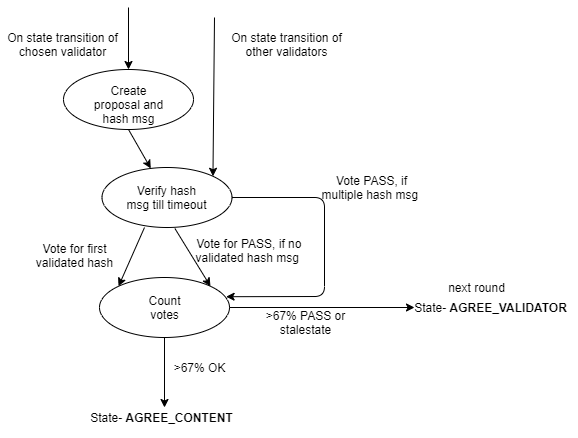
\includegraphics[width=100mm,scale=0.25]{figures/drawio/hash.png}
    \caption{AGREE HASH transition.}
    \label{fig:HASH}
\end{figure}


\begin{figure}
    \centering
    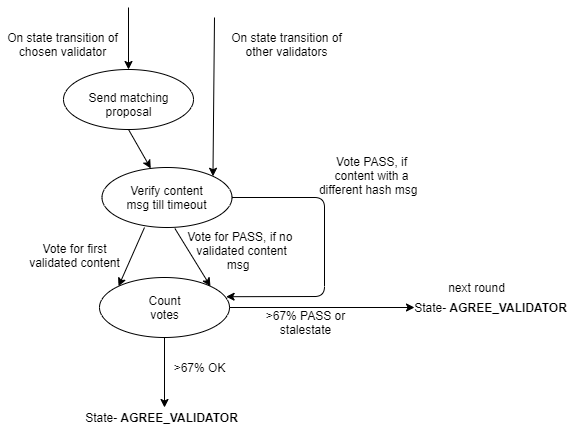
\includegraphics[width=100mm,scale=0.25]{figures/drawio/contents.png}
    \caption{AGREE CONTENT transition.}
    \label{fig:CONTENT}
\end{figure}

\subsection{Issues and Future work}
Given a chance, I would suggest the following improvements which can be made.
The checkpoint module performs well concerning the DAG's large size by calculating the summary in one repetition. The approach reduced the design complexity, but it is best to repeat the process after each transaction or transition if given a chance to improve it further. 
We want to emphasize testing the incentive mechanism while running the system for a long time as the incentive is the main reason for participating in the system and acting honestly.
